\chapter{SLAM}\label{chp:slam_mapping}

One of the first challenges in indoor navigation for assistive robots is actually finding where they are. Robot localization is fundamental to not only know where you need to go, but rather find a path there that avoids the obstacles.

Mapping is an essential tool in this matter, and it comprises the areas of \textit{concurrent mapping} and \textit{localization problem}. On themselves, both problems are relatively easy and well understood: mapping an environment knowing the localization and localizing the robot having the map in hands are simple tasks, however the combination of those two problems is hard to solve \cite{thrun2000real}.

Many SLAM (Simultaneous Localization and
Map Building) algorithms emerged to try and solve these problems, using different approaches and range of sensors to do the task. Some even evolved fusing data from different sensors to provide higher precision. They often rely on assumptions about the system nature. Most of the algorithms assume that the noise can be modeled  as a gaussian. Others might assume that the movement is linear and apply Kalman Filters to predict the current state.

\section{Sensors}

\subsection{Laser Scanners}

The laser scanner is one of the most simple ways to capture data about the environment. They work by sending beams of light in a direction and measuring the time it takes for the light to travel back and forth between the object and the sensor. As you want information to be gathered on more than a single point, the scanner can rotate a mirror or even the whole sensor to gather measurements from all directions, as shown on \prettyref{fig:sick_s300_diagram}. There are two main ways of measuring the object distance: time of flight and Phase-Shift \cite{amann2001laser}.

\begin{figure}
     \centering
     \subfloat[][]{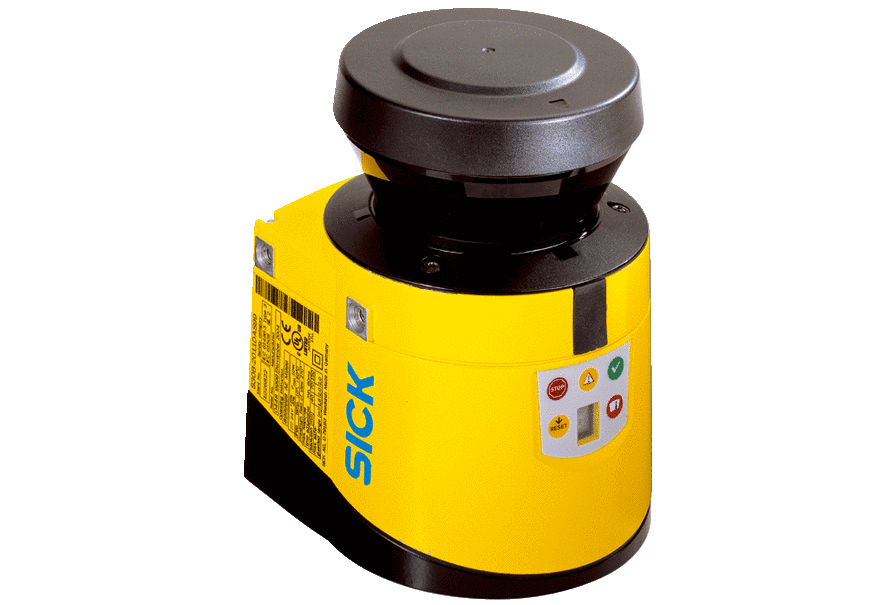
\includegraphics[width=80mm]{sick_s300}}
     \subfloat[][]{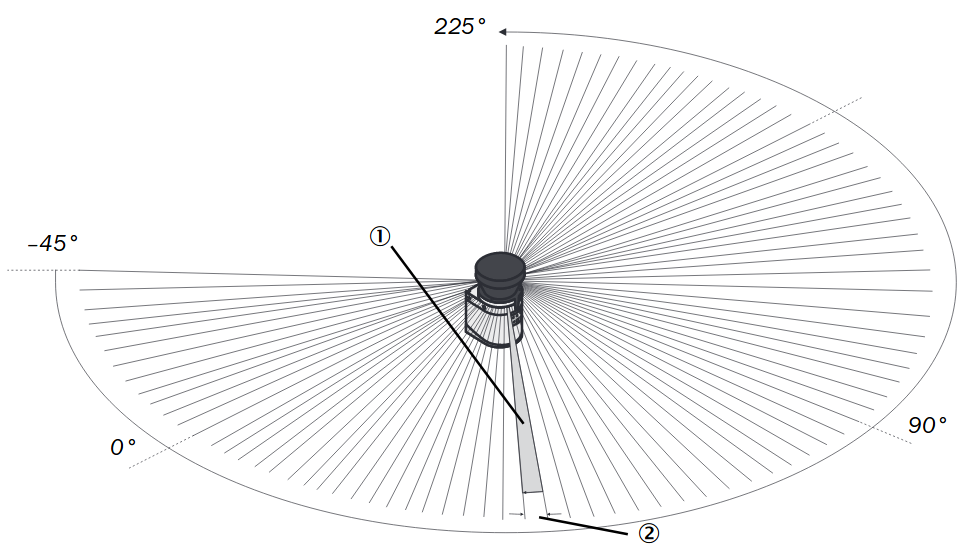
\includegraphics[width=80mm]{sick_s300_diagram}\label{fig:sick_s300_diagram}}
     \caption{SICK S300 Laser Scanner \cite{sicks300}.}
     \label{fig:sick_s300}
\end{figure}

In the time of flight measurement, a stopwatch is started when the beam of light is emitted. Since the speed of light is well known, the calculations are very straight forward, as shown on \prettyref{eq:d}. This form of measurement depends heavily on the quality of construction, as the usual sources of inaccuracy are noise (electronics, radiation in the room), timing (stopwatch precision, pulse detection), and minimal changes in each measurement can lead to big errors in the final result. Averaging and Filtering also take a big role in providing reliable data.

\begin{equation} \label{eq:d}
D = \frac{c \cdot t}{2}
\end{equation}

The second way of calculating the distance is by using phase-shift techniques, assuming there will be a difference in phase between the beam of light emitted and received. This varies according to the frequency and time traveled according to the equation $\phi = \omega \cdot t$, where $\phi$ is the phase-shift, $t$ the time traveled and $\omega$ the angular frequency of the wave. Isolating $t$ and substituting in \prettyref{eq:d}, we can derive the \prettyref{eq:d2} that dictates the distance based on frequency. This technique also requires more complex signal processing structures like a heterodyne for good for measurements.

\begin{equation} \label{eq:d2}
D = \frac{1}{2} \frac{c \cdot \phi}{\omega} = \frac{1}{4 \pi} \frac{c \cdot \phi}{f}
\end{equation}

\subsection{3D cameras}

Even though it is possible to recreate a 3D model of the environment using LIDAR laser scanners, discussed on the last subsection, those sensors coast thousands of dollars and are not very suited for robotics. Fortunately, it is possible to replace those sensors with 3D cameras capable of registering depth based on image processing techniques.

\section{Localizing the robot}

\subsection{Wheel Odometry}

Wheel odometry is one of the most simple ways to determine the position of the robot based on the starting point. Considering a flat surface, simply taking the turns made by each wheel and the steering actions, it is possible to estimate the path the robot took by applying the forward kinematics of the base.

The main disadvantages of wheel odometry are that the robot is limited to flat terrain, and even then slippery and small changes to forward kinematics (i.e. radius of the wheel changes slightly) can accumulate error over time.

\subsection{Laser Odometry}


\section{The localization and mapping problem}

The localization process can be expressed mathematically as follows \cite{thrun2005probabilistic}. Since all the measurements are discrete and supposing we want the localization of the robot through time, it can be represented as:

\begin{equation}\label{eq:x}
    X_t = \{x_0, x_1, \dots, x_t\} 
\end{equation}

The map can also be represented by a variable M as follows. Notice also that the map is considered to be time invariant in this case, and only depends on $n$ which is the number of features in the world.

\begin{equation}
    M = \{m_0, m_1, \dots, m_{n - 1}\}
\end{equation}

In order to do that, it is necessary to have some idea on how the robot is interacting with the world, how it is moving or the sensors readings. This can be for instance the measurements of robot odometry (wheel or laser odometry) or IMU data. The set of this measurements is defined as:

\begin{equation}
    U_t = \{u_0, u_1, \dots, u_t\}
\end{equation}

To also build the map, the robot will need the set of observations of the world, that can come as measurements from 3D cameras, LIDAR, SONAR, etc. This set of measurements is defined as:

\begin{equation}
    Z_t = \{z_0, z_1, \dots z_t\}
\end{equation}

Since every measurement in the robot is noise, the position can only be represented as a \textit{belief}, where the belief is the probability that the robot is in a position given the set of inputs and measurements. This can be represented as:
'
\begin{equation}
    bel(x_t, M) = p(x_t, M | u_{1, t}, z_{1,t})
\end{equation}

There are three main approaches to solve this problem, Extended Kalman Filters, Particle Filters and Graph based.

\subsection{Representing the map}

One of the concerns of mobile robots is how to build a map that is compatible with the environment and represents obstacles properly. While in some applications it is possible to have a pre-compiled map from the environment using the floor plan as a reference, those can be obsolete when dealing with highly dynamic environments or when objects get in the way. Even in static environments, there is a need to compensate for faulty or noise sensors, errors in localization, and the pre-compiled maps should only be used as complementary information. One of the techniques that emerged to solve these problems, and later was adopted as the core of many SLAM algorithms, is the Occupancy Grid \cite{elfes1989using} representation.

The Occupancy Grid is form of representing obstacles in 2D or 3D where each cell on the grid stores the probabilistic information of that area. This especially useful because it provides a comprehensive way to fuse sensor data, based on probability, instead of out-of-the-box algorithms that require fine tuning to work.

\begin{figure}[!ht]
    \centering
    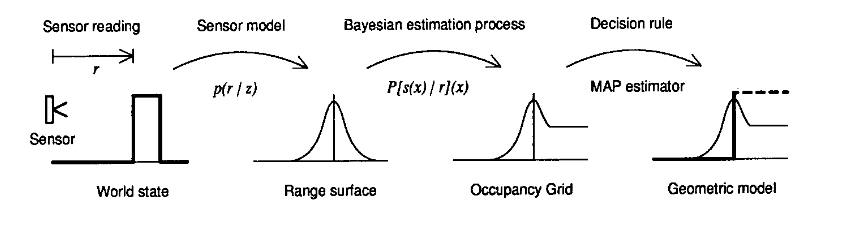
\includegraphics[width=.9\linewidth]{grid_steps}
    \caption{Steps when building an occupancy grid \cite{elfes1989using}.}
    \label{fig:grid_steps}
\end{figure}

According to \prettyref{fig:grid_steps}, the first step when building a sensor grid is to get the sensor reading. The next step is build a sensor model $p(r|z)$. Then, the Bayesian estimation is applied, based on all the observations before and current observations, to update the map. Finally, the world model is obtained using an estimator such as \textit{maximum a posteriori} (MAP). All those steps are done by the SLAM algorithms using different techniques, but even with default tuning those algorithms are good enough to work on most scenarios.

Naturally, the obstacle cell is labeled as occupied, with probability 1. All the cell until this one are labeled as empty, with probability 0. The unknown cells are labeled with unknown, with probability 0.5.

\begin{figure}[!ht]
    \centering
    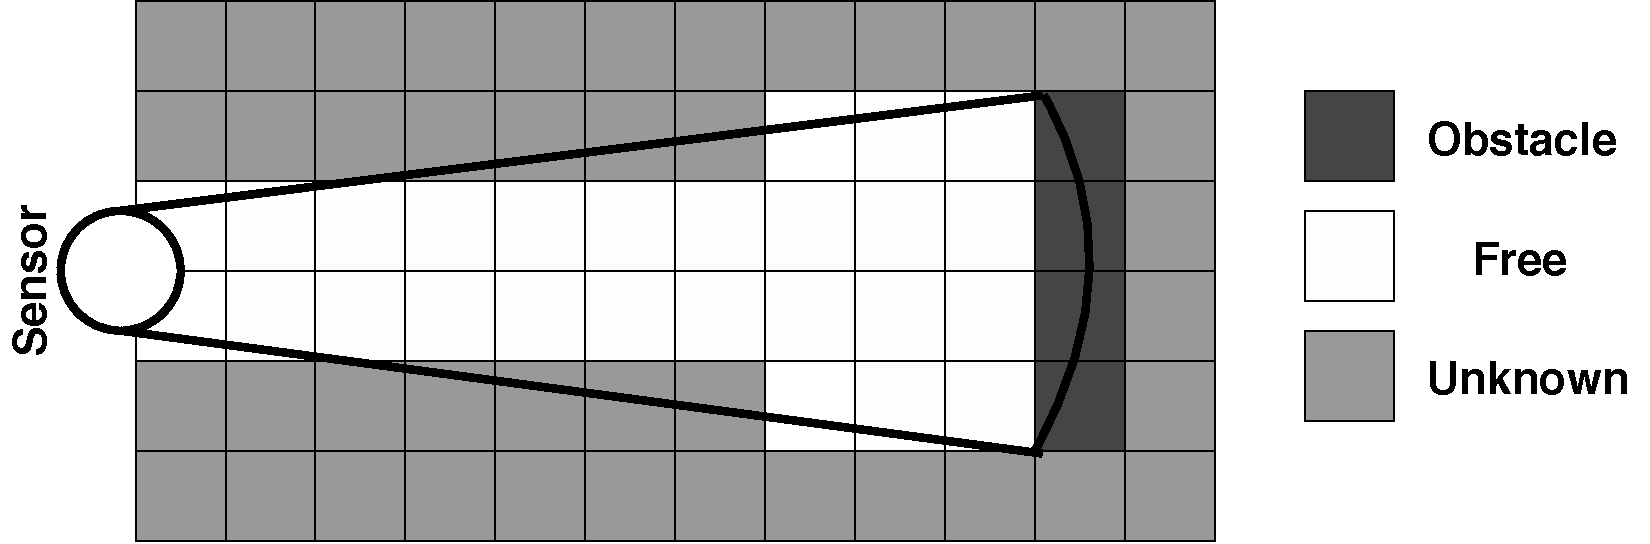
\includegraphics[width=.9\linewidth]{occupancy_grid}
    \caption{Occupancy grid for a single sensor.}
    \label{fig:occupancy_grid}
\end{figure}

The process is iterative and, as measurements from different points of view and different sensors grow, the maps become more and more complete, as shown on \prettyref{fig:occupancy_grid_algorithm}. The data fusion can also be done in different manners, but is commonly done using Kalman filters or Extended Kalman filters.

\begin{figure}[!ht]
    \centering
    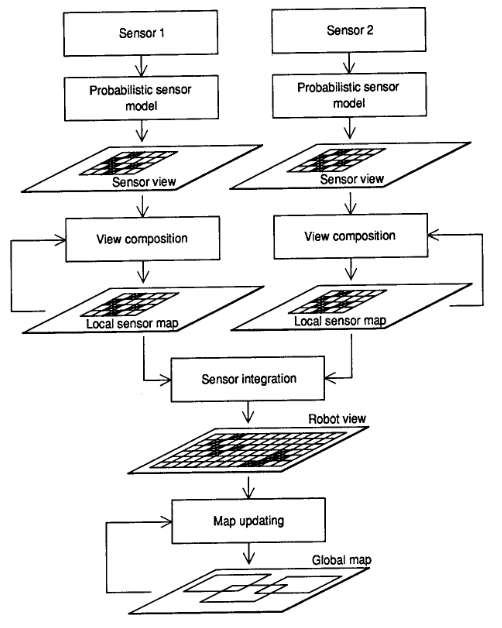
\includegraphics[width=.9\linewidth]{occupancy_grid_algorithm}
    \caption{Occupancy grid algorithm for multiple sensors.}
    \label{fig:occupancy_grid_algorithm}
\end{figure}

\section{ROS Slam Algorithms}

\subsection{Gmapping}

Gmapping is by far the most famous SLAM algorithm in robotics for a number of reasons. It was originally proposed by \citeauthor{doucet2000rao} in 2000 as way of using Particle filters algorithms with Rao-Blackwellized techniques. The main advantage of their approach is dealing with non-gaussian distributions that Kalman filters cannot deal with without rough linearization, as well as being less complex to implement.

\citeauthor{grisetti2007improved} in 2007 proposed improvements to \citeauthor{doucet2000rao} techniques in order to reduce complexity and make the resampling step better. It works by first reducing the amount of particles needed to be stored combining the current observation and odometry information, contrary to previous approaches where only odometry was used, reducing the estimation error and getting a more refined map. The second technique is using an adaptative resampling technique, meaning that resampling only has to be done when needed, reducing the problem with particle depletion, when only few particles are in high-probability areas and a lot of particles represent pretty old and unreliable information.

\subsection{Hector}

Hector SLAM first emerged in 2013 to solve the very specific problem of mapping in uneven terrains. It was aimed to be used in rescue robots that have to be robust enough to drive through ramps and obstacles and still be able to estimate the trajectory and map without reliable odometry information. Instead of trying to filter data to only include useful data, Hector pose estimation completely drops odometry data in favor of laser scanner data, and instead uses a fast LIDAR data scan-matching to estimate odometry. In order to estimate 6DOF, when moving in uneven terrain, the algorithm will also need a IMU device, and optional localization devices  like GPS, barometers and accelerometers. All the data is then fused using an Extended Kalman Filter (EKF), and not including odometry information is a simple way to exclude all errors caused by wheel spin, drift or slippery ground \cite{kohlbrecher2011flexible}.

\subsection{Karto}

Graph based SLAM closed source.

\subsection{Cartographer}

Cartographer is a fairly recent SLAM technique developed by Google. The concept behind the algorithm can be seen on \prettyref{fig:cartographer}. The main idea is separating the matters into two different problems: local SLAM and Global SLAM. The main objective is not having to deal with big maps or representations while mapping a new area. Instead, a submap is created for the local area and updated every new scan. Every scan is also tested against the submap using a Ceres-based scan matcher, to do pose optimization.

The idea of having submaps is that it is only build using a few scans, meaning that the estimate should be very close to reality. As the submaps grow larger, so does the error, meaning that every few scans a new submap is started. The Global SLAM thread will then have a collection of submaps to compute the whole map running loop closure \cite{cartographer2016google}.

\begin{figure}
    \centering
    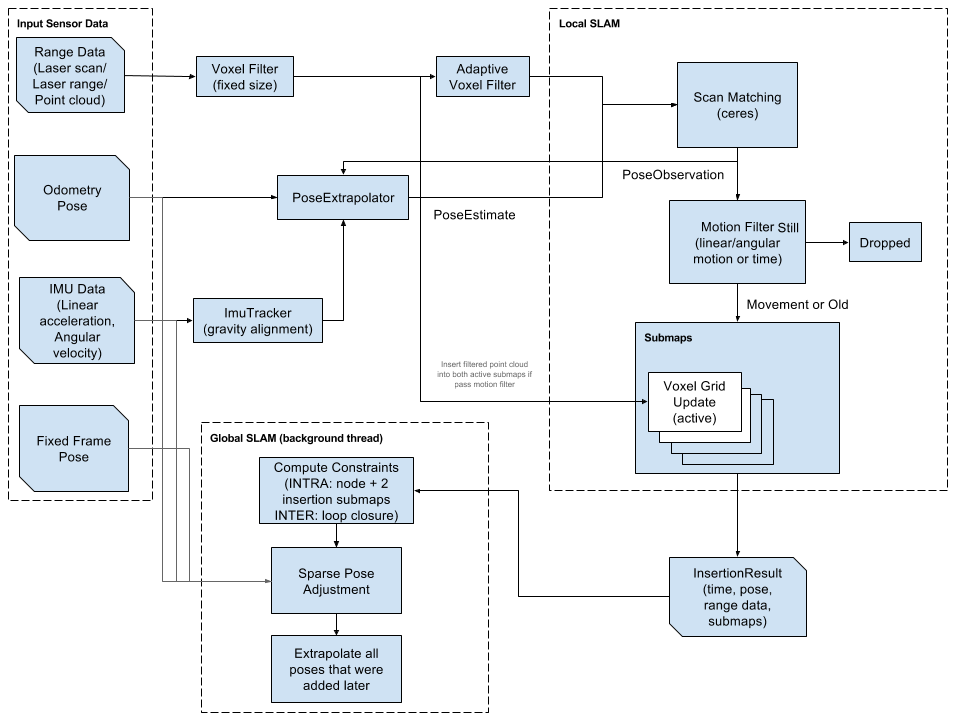
\includegraphics[width=0.6\linewidth]{cartographer}
    \caption{High-level System overview of Cartographer.}
    \label{fig:cartographer}
\end{figure}

\section{Evaluating SLAM Performance}

There is a lot of debate on how to evaluate SLAM performance. Since there are plenty of algorithms using different techniques, each one of the having their own set of parameters, there is a need to inspect them and tell which one does better in each scenario. A lot of this evaluation is done visually, assisted by a human that tells whether the occupancy grid is adequate considering the building floor plans. But as SLAM algorithms gets more precise, it is difficult to draw conclusions just from the appearance itself. Plus, there is the problem of not having the floor plants for publicly available datasets, making it harder to compare between methods \cite{kummerle2009measuring}.

According to \citeauthor{amigoni2007good}, the following issues have to be addressed when comparing SLAM:

\begin{itemize}
    \item The dataset must be pubicly available, examples being MIT Killian Court or the Intel Research Lab dataset.
    \item All algorithm parameters have to be indicated.
    \item The behavior for algorithm have to tested with different parameters in order to evaluate robustness.
    \item The dataset must include a closed-loop test, where the robot runs around an environment and comes back to the same place, to test against algorithm divergence.
    \item The ground truth must be used to evaluate results when available.
    \item Bad mapping results must be shown.
\end{itemize}

\citeauthor{kummerle2009measuring} proposes a framework to analyze mapping accuracy using satellite imagery, but uses visual inspection in order to estimate the relations between the robot poses and the environment. The estimation is then compared to the SLAM results and the final metric is the "deformation energy" required to transform the mapped result into ground truth. In other words, each of the $N$ displacements $\delta_{i,j}$ is compared against the ground truth $\delta_{i,j}^*$ using the \prettyref{eq:displacement}, for a set of  $(i,j)$ pairs.

\begin{equation}\label{eq:displacement}
    \epsilon(\delta) = \frac{1}{N} \sum_{i, j} trans(\delta_{i,j} \ominus \delta_{i,j}^*)^2 + rot(\delta_{i,j} \ominus \delta_{i,j}^*)^2
\end{equation}

 The displacement $\delta_{i, j}$ is simply calculated by the the transformation between a local measurement between two known poses, from pose $i$ to pose $j$, as described in \prettyref{eq:x}. Evaluating the displacement instead of the global position is great because it makes the evaluation resilient to small errors at the start of mapping that would impact every subsequent global position, even when the mapping in the next steps is done correctly. Since the ground-truth displacement is not available, this implementation relies on the fact that the relation between two poses can be calculated using the laser scanner, each pose later evaluated by a human. It also relies on a good enough initial guess, also human assisted. The authors also assume just evaluating the poses without evaluating the resulting map is enough for SLAM benchmarking. While this hold true for most cases, it is still very hard to infer global performance, as global displacements (large enough distance between $i$ and $j$) also carry the problem of accumulating human error.
 
 \citeauthor{santos2013evaluation} proposes a more in-depth comparison with the publicly available SLAM algorithms that run on ROS. The authors ran both noise-free simulation and real-life experiments with the scenarios and analyzed the error metric between the ground-truth map and the generated map, also evaluating the CPU usage for each algorithm. The authors however didn't provide extensive information on how the maps were aligned, very important since the fit has to be optimal in order to do adequate comparison.